% When submitting your files, remember to upload this *tex file, the pdf generated with it, the *bib file (if bibliography is not within the *tex) and all the figures.
%%%%%%%%%%%%%%%%%%%%%%%%%%%%%%%%%%%%%%%%%%%%%%%%%%%%%%%%%%%%%%%%%%%%%%%%%%%%%%%%%%%%%%%%%%%%%%%%%%%%%%%%%%%%%%%%%%%%%%%%%%%%%%%%%%%%%%%%%%%%%%%%%%%%%%%%%%%

%%% Version 3.3 Generated 2016/11/10 %%%
%%% You will need to have the following packages installed: datetime, fmtcount, etoolbox, fcprefix, which are normally inlcuded in WinEdt. %%%
%%% In http://www.ctan.org/ you can find the packages and how to install them, if necessary. %%%
%%%  NB logo1.jpg is required in the path in order to correctly compile front
%%%  page header %%%

%% Bias in longitudinal cohort studies
%% Author: Denis Haine
%% Research topic
%% Date: 20170818
%% To compile:
%%  Rscript -e "library(knitr); knit('file.Rnw')"
%%  pdflatex file.tex
%%  bibtex file
%%  pdflatex file.tex
%%  pdflatex file.tex
%%
%% bibexport -o extracted.bib myarticle.aux
%%===============================================================

\documentclass[utf8]{frontiersSCNS}\usepackage[]{graphicx}\usepackage[]{color}
%% maxwidth is the original width if it is less than linewidth
%% otherwise use linewidth (to make sure the graphics do not exceed the margin)
\makeatletter
\def\maxwidth{ %
  \ifdim\Gin@nat@width>\linewidth
    \linewidth
  \else
    \Gin@nat@width
  \fi
}
\makeatother

\usepackage{Sweavel}

 % for Science, Engineering and Humanities and Social Sciences articles
%\documentclass[utf8]{frontiersHLTH} % for Health articles
%\documentclass[utf8]{frontiersFPHY} % for Physics and Applied Mathematics and Statistics articles
\usepackage[utf8]{inputenc}
\usepackage[T1]{fontenc}
\usepackage[english]{babel}

%\setcitestyle{square} % for Physics and Applied Mathematics and Statistics articles
\usepackage{url,hyperref,lineno,microtype,subcaption}
\usepackage[onehalfspacing]{setspace}

\usepackage{graphicx}
\usepackage{amsmath}
\usepackage{relsize}
\usepackage{amssymb}  % for math symbols
\usepackage{mathtools}  % mathtools builds on and extends amsmath package
\usepackage{moreverb}
\usepackage{xspace}
\usepackage{booktabs}
\usepackage{xfrac}
\usepackage{cleveref}
\usepackage{paralist}  % for in-line list
\usepackage{siunitx}
\usepackage[autolanguage]{numprint}
\usepackage[super]{nth}  % to generate English ordinal numbers

\newcommand{\code}[1]{\texttt{\smaller #1}}
\newcommand{\R}{{\normalfont\textsf{R}}{}}


\linenumbers


% Leave a blank line between paragraphs instead of using \\


\def\keyFont{\fontsize{8}{11}\helveticabold }
\def\firstAuthorLast{Haine {et~al.}} %use et al only if is more than 1 author
\def\Authors{Denis Haine\,$^{1,3,*}$, Ian Dohoo\,$^{2,3}$ and Simon Dufour\,$^{1,3}$}
% Affiliations should be keyed to the author's name with superscript numbers and be listed as follows: Laboratory, Institute, Department, Organization, City, State abbreviation (USA, Canada, Australia), and Country (without detailed address information such as city zip codes or street names).
% If one of the authors has a change of address, list the new address below the correspondence details using a superscript symbol and use the same symbol to indicate the author in the author list.
\def\Address{$^{1}$Faculté de médecine vétérinaire, Université de Montréal, St-Hyacinthe, QC, Canada \\
$^{2}$Centre for Veterinary Epidemiological Research, Atlantic Veterinary
College, University of Prince Edward Island, Charlottetown, PE, Canada \\
$^{3}$Canadian Bovine Mastitis and Milk Quality Research Network, St-Hyacinthe,
QC, Canada}
% The Corresponding Author should be marked with an asterisk
% Provide the exact contact address (this time including street name and city zip code) and email of the corresponding author
\def\corrAuthor{Simon Dufour}

\def\corrEmail{simon.dufour@umontreal.ca}


\graphicspath{{graphics/pdf/}}

\newcommand{\rmm}{3.4.3}

\begin{document}
\onecolumn
\firstpage{1}

\title[Bias in Cohort Studies]{Selection and Misclassification Biases in
  Longitudinal Studies} 

\author[\firstAuthorLast ]{\Authors} %This field will be automatically populated
\address{} %This field will be automatically populated
\correspondance{} %This field will be automatically populated

\extraAuth{}% If there are more than 1 corresponding author, comment this line and uncomment the next one.
%\extraAuth{corresponding Author2 \\ Laboratory X2, Institute X2, Department X2, Organization X2, Street X2, City X2 , State XX2 (only USA, Canada and Australia), Zip Code2, X2 Country X2, email2@uni2.edu}


\maketitle


\begin{abstract}

%%% Leave the Abstract empty if your article does not require one, please see the Summary Table for full details.
  \section{}
Using imperfect tests may lead to biased estimates of disease frequency and
measures of association.
Many studies have looked into the effect of misclassification on statistical
inferences.
These evaluations were either within a cross-sectional study framework,
assessing biased prevalence, or for cohort study designs, evaluating biased
incidence rate or risk ratio estimates based on misclassification at one
of the two time-points (initial assessment or follow-up).
However, both observations at risk and incident cases can be wrongly
identified in longitudinal studies, leading to selection and misclassification
biases, respectively.
The objective of this paper was to evaluate the relative impact of selection
and misclassification biases resulting from misclassification, together, on
measures of incidence and risk ratio.

To investigate impact on measure of disease frequency, data sets from a
hypothetical cohort study with two samples collected one month apart were
simulated and analyzed based on specific test and disease characteristics, with
no elimination of disease during the sampling interval or clustering of
observations.
Direction and magnitude of bias due to selection, misclassification, and total
bias was assessed for diagnostic test sensitivity and specificity ranging from
0.7 to 1.0 and 0.8 to 1.0, respectively, and for specific disease contexts,
i.e.\ disease prevalences of 5 and 20\%, and disease incidences of 0.01, 0.05,
and 0.1 cases/animal-month.
A hypothetical exposure with known strength of association
was also generated.
A total of \numprint{1000} cohort studies of \numprint{1000} observations each
were simulated for these six disease contexts where the same diagnostic test
was used to identify observations at risk at beginning of the cohort and
incident cases at its end.

Our results indicated that the departure of the estimates of disease incidence
and risk ratio from their true value were mainly a function of test
specificity, and disease prevalence and incidence.
The combination of the two biases, at baseline and follow-up, revealed the
importance of a good to excellent specificity relative to sensitivity for the
diagnostic test.
Small divergence from perfect specificity extended quickly to disease
incidence over-estimation as true prevalence increased and true incidence
decreased.
A highly sensitive test to exclude diseased subjects at baseline was of less
importance to minimize bias than using a highly specific one at baseline.

Near perfect diagnostic test attributes were even more important to obtain a
measure of association close to the true risk ratio, according to specific
disease characteristics, especially its prevalence.
Low prevalent and high incident disease lead to minimal bias if disease is
diagnosed with high sensitivity and close to perfect specificity at baseline and
follow-up.
For more prevalent diseases we observed large risk ratio biases towards the
null value, even with near perfect diagnosis.

% For full guidelines regarding your manuscript please refer to \href{http://www.frontiersin.org/about/AuthorGuidelines}{Author Guidelines}.

\tiny
 \keyFont{ \section{Keywords:} bias (epidemiology), longitudinal study,
   selection bias, misclassification, epidemiologic methods} %All article types: you may provide up to 8 keywords; at least 5 are mandatory.
\end{abstract}



%------------------
\def\inclcode{1}


\section{Introduction}

A cohort study is a longitudinal observational study in which a study population
(i.e.\ a cohort)  is selected and followed up in
time~\citep{DosSantosSilva1999,Rothman2012}.
Members of the cohort share a common experience (e.g. Kennel Club registered
Labrador Retrievers born after January \nth{1}, 2010; \citealp{Clements_2013}) or
condition (e.g.\ litters from \emph{A.\ pleuropneumoniae} infected sows; \citealp{Tobias_2014}).
Two cohorts are often included in these longitudinal studies, one experiencing a
putative causal event or condition (exposed cohort), and the other being an
unexposed (reference) cohort.
Cohort study is the standard study design to estimate the incidence of diseases
and identify their natural history, by analyzing the association between a
baseline exposure and risk of disease over the follow-up period.
This type of study is characterized by the identification of a disease-free
population (i.e.\ subjects with the outcome at baseline are excluded from the
follow-up), and their exposure to a risk factor is assessed.
The frequency of the outcome (generally the incidence of a disease or death) is
measured and related to exposure status, expressed as a risk ratio (RR).
Therefore it is assumed that prevalent and non-prevalent cases can be
differentiated with no error so that only susceptible individuals are included
in the cohort.
Incident cases are likewise supposed to be correctly identified.

However, any measurement is prone to potential errors, as a result of subjective
evaluations, imperfect diagnostic tests, reporting errors (deliberate or not),
recall deficiencies, or clerical errors.
Obtaining ``error-free'' measurements is a desirable objective but it is
usually much more expensive to use ``gold-standard'' measurements, or they
are simply not available, leaving the researcher with ``less-than-ideal''
measurement tools.
Wrong classification at baseline and at follow-up are both misclassification
biases, in the former the bias resulting from misclassification could be
considered a selection bias, as the wrong (diseased) subjects are included in
the cohort~\citep{Rothman2012} while in the latter, it would be commonly defined
as misclassification bias~\citep{Delgado-Rodriguez2004}.
Such errors of measurement or misclassification in exposure variables, outcomes
or confounders can bias inferences drawn from the data collected, often
substantially~\citep{Quade1980}, or decrease the power of the
study~\citep{Bross1954,WHITE_1986}.
Many studies have looked into the effect of misclassification on statistical
inferences, including biased prevalence and incidence rate
estimates~\citep{Rogan1978,Quade1980} and biased relative risk
estimates~\citep{Barron1977,Greenland1980}.
Nondifferential misclassification of disease leads in general to bias towards
null in the estimated associations as well as reduced statistical
efficiency~\citep{Bross1954,Barron1977,Copeland1977}.
This bias depends mainly on the specificity (Sp) of the test
used~\citep{Copeland1977}.
If Sp of the test is perfect, then bias is absent~\citep{Poole1985}.
These evaluations were, however, either within a cross-sectional study
framework, assessing biased prevalence, or for cohort study designs evaluating
biased incidence rate or RR estimates but based on misclassification at only one
of the two time-points (initial assessment or follow-up).
However, both observations at risk and incident cases can be wrongly identified
in longitudinal studies, leading to selection and misclassification biases,
respectively.

The objective of this paper was to evaluate the relative impact of selection and
misclassification biases resulting from misclassification, together, on measures
of incidence and RR.

\section{Material and Methods}

To investigate the impact of concomitant selection and misclassification biases
on measure of disease frequency, data sets from a hypothetical cohort study with
two samples collected one time unit apart were simulated and analyzed based on
specific test and disease characteristics, for a stable population over the
follow-up time, and with no elimination of disease or clustering of
observations.
Direction and magnitude of bias due to selection, misclassification, and total
bias was assessed for diagnostic test sensitivity (Se) and Sp 
ranging from 0.7 to 1.0 (0.7, 0.75, 0.8, 0.85, 0.9, 0.95, 0.98, 0.99, 1) and 0.8
to 1.0 (0.8, 0.85, 0.9, 0.95, 0.98, 0.99, 1), respectively, and for specific
disease contexts, i.e.\ disease prevalences of 5 and 20\%, and disease
incidences of 0.01, 0.05, and 0.1 cases/animal-time unit.
The true case status (\(S_1\)) on first sample collection was used to identify
observations at risk at the beginning of the cohort, while the second (\(S_2\))
was used to identify the true outcome.
A hypothetical exposure with known strength of association (RR
\raise.17ex\hbox{$\scriptstyle\sim$}\num{3.0}) was also generated.
For demonstration purpose, simulations were also ran with a weaker RR of
\raise.17ex\hbox{$\scriptstyle\sim$}\num{1.5} (Supplementary Material).
A total of \numprint{1000} cohort studies of \numprint{1000} observations each
were simulated for these six disease contexts where the same diagnostic test was
used to identify observations at risk at beginning of the cohort and incident
cases at its end.
On each datasets new \(S_{1}'\) and \(S_{2}'\) variables were generated by
applying the scenario misclassification parameters to the \(S_1\) and \(S_2\)
samples.
Incidence and measures of association with the hypothetical exposure were then
computed using first the \(S_{1}'\) and \(S_{2}'\) variables (total bias), then
\(S_{1}'\) and \(S_2\) (selection bias only), and finally the \(S_1\) and
\(S_{2}'\) variables (misclassification bias only).

Disease incidence was computed as the number of new cases at the end of the
cohort divided by the number at risk at its beginning.
Risk ratio was computed as the  ratio of the risk of disease among observations
who were exposed to the risk factor, to the risk among observations who were
unexposed~\citep{Rothman2012}.
Data sets generation and estimation procedures were realized in
\R~\citep{Rsystem}, and simulation code is available at
\url{https://github.com/dhaine/cohortBias}.

\section{Results}
\label{sec:results}

Total biases resulting from selection and misclassification errors and according
to given disease prevalence, Se, and Sp are illustrated for disease incidence
and RR in \Cref{fig:incidence_contour,fig:incidence_risk}, respectively.
These figures are contour plots where the lines are curves in the \(x, y\)-plane
along which the function of the two variables on the vertical and horizontal
axes (i.e.\ Se and Sp) has a constant value, i.e.\ a curve joins points of equal
value~\citep{courant_1996}.
The true incidence rate (or RR) is therefore to be found at the upper right
corner of the plot.
For example, in the bottom left panel of \Cref{fig:incidence_contour} the second
line from the bottom is labelled 0.22.
This line shows that, for a 5\% disease prevalence and a true incidence rate of
0.1 case/animal-time unit, an apparent incidence estimate of 0.22 will be
achieved by any combination of Sp and Se on this line (e.g.\ Sp = 0.845, Se =
0.7 or Sp = 0.87 and Se = 1.00).
As an other example, in the upper right panel of this same figure, the first
line at the top is labelled 0.02.
It shows that, for a 5\% disease prevalence and a true incidence rate of 0.01
case/animal-time unit, an apparent incidence estimate of 0.02 is achieved along
this line by any combination of Se and Sp like, for example, a Sp of 1.00 and a
Se of 0.955. The true incidence rate is given at the upper right corner, where
Se and Sp are both 100\%.
Imperfect Se to identify individuals at risk at baseline and imperfect Sp to
identify incident cases led to a mild under-estimation of the observed disease
incidence (Figures~S1 and S2 in Supplementary Material).
From these graphs we could also note that Sp has little effect on selection bias
while Se has little effect on misclassification bias.
Of the two, misclassification bias had a much bigger effect than selection bias.
But overall, the combination of the two biases, at baseline and follow-up,
revealed the importance of a good to excellent Sp relative to Se for the
diagnostic test.
Small divergence from perfect Sp extended quickly to disease incidence
over-estimation as true prevalence increased and true incidence decreased
(\Cref{fig:apparent_incidence_5,fig:apparent_incidence_20,fig:apparent_RR}).
Selection and misclassification biases of a low prevalent and incident disease,
diagnosed with close to perfect Sp, were minimal, reflecting the importance of
choosing a highly specific test to improve identification of animal (or
individual) unit at risk and incident case identification.
The same effect was also observed with RR estimations (Figures~S3 and S4).
Similar results were found with a weaker exposure, RR of 1.5 (Figures~S5 to S8).

\section{Discussion}
\label{sec:discussion}

Our results indicated that the departure of the estimates of disease incidence
and risk ratio from their true value were mainly a function of test Sp, and
disease prevalence and incidence.
Imperfect Se to identify individuals at risk and imperfect Sp to identify
incident cases led to a mild under-estimation of the observed disease incidence.
The combination of the two biases, at baseline and follow-up, revealed the
importance of a good to excellent Sp (over 95\%) over Se for the diagnostic
test.
Small divergence from perfect Sp extended quickly to disease incidence
over-estimation as true prevalence increased and true incidence decreased.
Selection and misclassification biases of a low prevalent and incident
disease, diagnosed with close to perfect Sp, were minimal, reflecting the
importance of choosing a highly specific test to improve unit at risk and case
identification.
A highly sensitive test to exclude diseased subjects at baseline was of less
importance to minimize bias than using a highly specific one at this time point.
Of course, the situation would be different in a population with a very high
disease prevalence.
For most diseases, however, the tendency is to have a large proportion of
healthy animals and a small proportion of diseased ones.
The range of diseases prevalence investigated in our study (5--20\%) would
therefore cover most disease scenarios seen in veterinary, and perhaps, human
studies.

Near perfect diagnostic test attributes were even more important to obtain a
measure of association close to the true risk ratio, according to specific
disease characteristics, especially its prevalence.
Low prevalent and high incident disease led to minimal bias if disease was
diagnosed with high Se and close to perfect Sp.
For more prevalent diseases we observed large risk ratio biases towards the
null value, even with near perfect diagnosis.
This bias also got larger as incidence decreased.
For diseases with moderate to high prevalence (20\%), the biases could be so
important that a study using a test with a Se or Sp < 0.95
would have very little power to identify any measure of association with
exposures.
Even with prevalence of disease of 5\%, a dramatic loss of power is to be
expected when imperfect tests are used.
Therefore a corollary result of a sub-optimal Sp is that, by causing a bias
towards the null, weaker associations (like our RR
\raise.17ex\hbox{$\scriptstyle\sim$}\num{1.5}) will be more difficult to
demonstrate.
It would be unnecessary to fight this loss in power by increasing the study
sample size in order to get a narrower confidence interval, as the measured
association would be biased anyway~\citep{Brenner_1990}.
It was already demonstrated that study power decreases as misclassification
increases~\citep{Brown_2010}.
For stronger associations and in the presence of small biases, sample size could
be adjusted~\citep{Dendukuri_2004,Cheng_2009}.
But in the presence of larger biased associations towards the null, a weaker,
reduced, association would be candidate for further investigation, even if its
confidence interval includes \num{1.0}~\citep{Baird_1991}.

It is already recognized that misclassification of outcome or exposure during
follow-up leads to bias towards null in the estimated
associations~\citep{Bross1954,Copeland1977,FLEGAL_1986} as well as reduced
statistical efficiency by loss of power~\citep{WHITE_1986} and confidence
intervals of the parameters estimates that are too narrow~\citep{Neuhaus_1999}.
However this bias towards the null value is strictly true only when
misclassification is the same in the two compared groups, i.e.\ exposure and
covariates status do not influence Se and/or
Sp~\citep{Copeland1977,Sorahan_1994,Neuhaus_1999}.
In this case, we have non-differential misclassification.
As shown previously by \cite{Copeland1977}, misclassification bias depends
primarily on the Sp of the test used and increase with disease rarity, with most
of the bias occurring even before the Sp drops below 85\%.
With Se and Sp as high as 0.90 and 0.96, respectively, RR is already
substantially biased (1.5 instead of 2)~\citep{Copeland1977}, but when Sp is
perfect, bias is absent~\citep{Poole1985}.
When disease frequency is low, error in disease diagnosis leads to an increase
in false positives which submerge true positives and dilute measures of
incidence and association.
Bias in RR increases as Se increase and Sp decrease~\citep{WHITE_1986}.
Exposure misclassification alone can cause serious bias on the RR even if Se or
Sp are not lower than 80\%~\citep{Kristensen_1992}.

When misclassification is differential, i.e.\ Se and Sp of outcome
classification is not equal in each true category of exposure (or Se and Sp of
exposure classification is not equal in each true category of outcome),
direction of bias for parameter estimates can be in any
direction~\citep{Dosemeci_1990,Neuhaus_1999,Chen_2013}.
In this case, Se and Sp as low as 90\% can be sufficient to produce high
bias~\citep{Kristensen_1992}.
Direction of the bias can also be in any direction with dependent
misclassification (i.e.\ the errors in one variable are associated with the
errors in an other, \citealp{Assakul_1967,Greenland_1989}), even if
non-differential~\citep{Kristensen_1992}.
The same is found when the exposure variable is not dichotomous but has multiple
levels~\citep{Dosemeci_1990,Weinberg_1994}.
Bias towards the null also requires that selection bias and confounding are
absent~\citep{Jurek_2004}.
There are therefore many situations where bias towards null do not apply.
Even when non-differential misclassification is thought to take place, random
errors in the observed estimates can lead bias away from the
null~\citep{Jurek_2004}.

In cohort studies, non-differential misclassification of disease at baseline,
i.e.\ selection bias, especially imperfect Se, can lead to over- or
under-estimation of the observed RR~\citep{Pekkanen2006}.
This bias can be significant for disease with a low true incidence, a high true
prevalence, a substantial disease duration (i.e.\ as long as the interval between
first and second test), and a poor test Se.
In the presence of misclassification of disease at baseline the observed RR
depend on the association between exposure and disease both at baseline and
during follow-up~\citep{Pekkanen2006}.
Therefore to minimize bias, the standard recommendation is to exclude subjects
with the outcome at baseline from the cohort based on a highly sensitive
test~\citep{Pekkanen2008}.
Then during the follow-up period, case identification should use a highly
specific test having a high positive predictive value~\citep{Brenner1993}.
However \cite{Haine2017} have shown that a more prevalent and incident disease
diagnosed with an imperfect Se and/or Sp will give biased measure of association
despite attempts to improve its diagnosis.

We have shown here that combined misclassification at baseline and follow-up
requires a highly specific test.
If a test with high Sp cannot be used, one could use a less efficient test twice
at recruitment or for identifying incident cases and with a serial
interpretation.
The loss in Se of such an approach would cause little bias, compared to the
potential gains due to the increased Sp.
However, this combined misclassification would also require a highly sensitive
test to estimate an association close to the true RR.
Unfortunately increasing Sp of a test very often decreases its Se, i.e.\ a lower
probability for diseased individuals to be recognized as diseased.
As a results, some classification errors are to be expected leading to biased
parameters estimates.
If classification errors cannot be avoided during the study design stage, the
misclassification bias can be corrected into the analytic stage.
For instance, Se and Sp of the test can be incorporated into the modelling
strategy~\citep{Magder1997}, by performing a probabilistic sensitivity
analysis~\citep{Fox_2005}, or by including the uncertainty in the estimates with
a Bayesian analysis in the form of prior distributions~\citep{McInturff2004}.
A latent class model~\citep{Hui1980} would therefore return the posterior
inference on regression parameters and the Se and Sp of both tests.
Acknowledgement of these biases and possible corrective measures are important
when designing longitudinal studies when gold standard measurement of the
outcome might not be readily available, like for bacterial diseases (for example
subclinical intramammary infection; \citealp{Koop2013}), viral
diseases~\citep{Dotti2013} or more complex outcome evaluations (e.g.\ bovine
respiratory disease complex; \citealp{Buczinski2015}).
Efforts should be made to improve outcome evaluation but absence or limitation of
bias is not always granted in some situation.
\cite{Haine2017} demonstrated that for some specific disease incidences and
prevalences bias could not be avoided by improving outcome measurements.
Using latent class models can help in these cases, as shown by \cite{Dufour2012}.

Bias in parameters estimates can be important when considering selection and
misclassification biases together in a cohort study.
Our results underscore the need for a careful evaluation of the best available
options to identify at risk and incident cases according to the expected disease
prevalence and incidence of the study. 

\section*{Conflict of Interest Statement}

The authors declare that the research was conducted in the absence of any
commercial or financial relationships that could be construed as a potential
conflict of interest.

\section*{Author Contributions}

DH conducted the simulations, data analysis, results interpretation, and the
manuscript writing.
ID and SD contributed in interpreting the results and editing the manuscript.
DH, ID, and SD contributed to the planning of the study.

\section*{Funding}

This research was financed by the senior author (SD) Natural Sciences and
Engineering Research Council of Canada Discovery Grant.

% \section*{Acknowledgments}
% This is a short text to acknowledge the contributions of specific colleagues,
% institutions, or agencies that aided the efforts of the authors.

\section*{Supplementary Figures}

\textbf{Figure S1.} Estimated incidence rate as a function of test sensitivity
and specificity, a disease prevalence of 5\%, and true disease incidence (0.01,
0.05, 0.1 case/animal-time unit) when using an imperfect test at baseline
(selection bias) or at follow-up (misclassification bias). True incidence rate
is found at the upper right corner (i.e.\ perfect sensitivity and specificity).
\textbf{Figure S2.} Estimated incidence rate as a function of test sensitivity
and specificity, a disease prevalence of 20\%, and true disease incidence (0.01,
0.05, 0.1 case/animal-time unit) when using an imperfect test at baseline
(selection bias) or at follow-up (misclassification bias). True incidence rate
is found at the upper right corner (i.e.\ perfect sensitivity and specificity).
\textbf{Figure S3.} Estimated risk ratio as a function of test sensitivity and
specificity, a disease prevalence of 5\%, and true disease incidence (0.01,
0.05, 0.1 case/animal-time unit) for an exposure with a true measure of
association corresponding to a risk ratio of \(3.0\) when using an imperfect
test at baseline (selection bias) or at follow-up (misclassification bias). True
risk ratio is found at the upper right corner (i.e.\ perfect sensitivity and
specificity).
\textbf{Figure S4.} Estimated risk ratio as a function of test sensitivity and
specificity, a disease prevalence of 20\%, and true disease incidence (0.01,
0.05, 0.1 case/animal-time unit) for an exposure with a true measure of
association corresponding to a risk ratio of \(3.0\) when using an imperfect
test at baseline (selection bias) or at follow-up (misclassification bias). True
risk ratio is found at the upper right corner (i.e.\ perfect sensitivity and
specificity).
\textbf{Figure S5.} Estimated risk ratio as a function of test sensitivity and
specificity, disease prevalence (5 or 20\%), and true disease incidence (0.01,
0.05, 0.1 case/animal-time unit) for an exposure with a true measure of
association corresponding to a risk ratio of \(1.5\) when using an imperfect
test both at baseline and follow-up (i.e.\ total bias). True risk ratio is found
at the upper right corner (i.e.\ perfect sensitivity and specificity).
\textbf{Figure S6.} Estimated risk ratio as a function of test specificity and
disease risk, and for a sensitivity of 95\%, when using an imperfect test both
at baseline and follow-up. True risk ratio = \(1.5\).
\textbf{Figure S7.} Estimated risk ratio as a function of test sensitivity and
specificity, a disease prevalence of 5\%, and true disease incidence (0.01,
0.05, 0.1 case/animal-time unit) for an exposure with a true measure of
association corresponding to a risk ratio of \(1.5\) when using an imperfect
test at baseline (selection bias) or at follow-up (misclassification bias). True
risk ratio is found at the upper right corner (i.e.\ perfect sensitivity and
specificity).
\textbf{Figure S8.} Estimated risk ratio as a function of test sensitivity and
specificity, a disease prevalence of 20\%, and true disease incidence (0.01,
0.05, 0.1 case/animal-time unit) for an exposure with a true measure of
association corresponding to a risk ratio of \(1.5\) when using an imperfect
test at baseline (selection bias) or at follow-up (misclassification bias). True
risk ratio is found at the upper right corner (i.e.\ perfect sensitivity and
specificity).

\bibliographystyle{frontiersinSCNS_ENG_HUMS} % for Science, Engineering and Humanities and Social Sciences articles, for Humanities and Social Sciences articles please include page numbers in the in-text citations
%\bibliographystyle{frontiersinHLTH&FPHY} % for Health, Physics and Mathematics articles
\bibliography{bias}

%%% Make sure to upload the bib file along with the tex file and PDF
%%% Please see the test.bib file for some examples of references

\section*{Figure captions}

%%% Please be aware that for original research articles we only permit a combined number of 15 figures and tables, one figure with multiple subfigures will count as only one figure.
%%% Use this if adding the figures directly in the mansucript, if so, please remember to also upload the files when submitting your article
%%% There is no need for adding the file termination, as long as you indicate where the file is saved. In the examples below the files (logo1.jpg and logos.jpg) are in the Frontiers LaTeX folder
%%% If using *.tif files convert them to .jpg or .png
%%%  NB logo1.jpg is required in the path in order to correctly compile front page header %%%

\begin{figure}[htbp]
  \begin{center}
    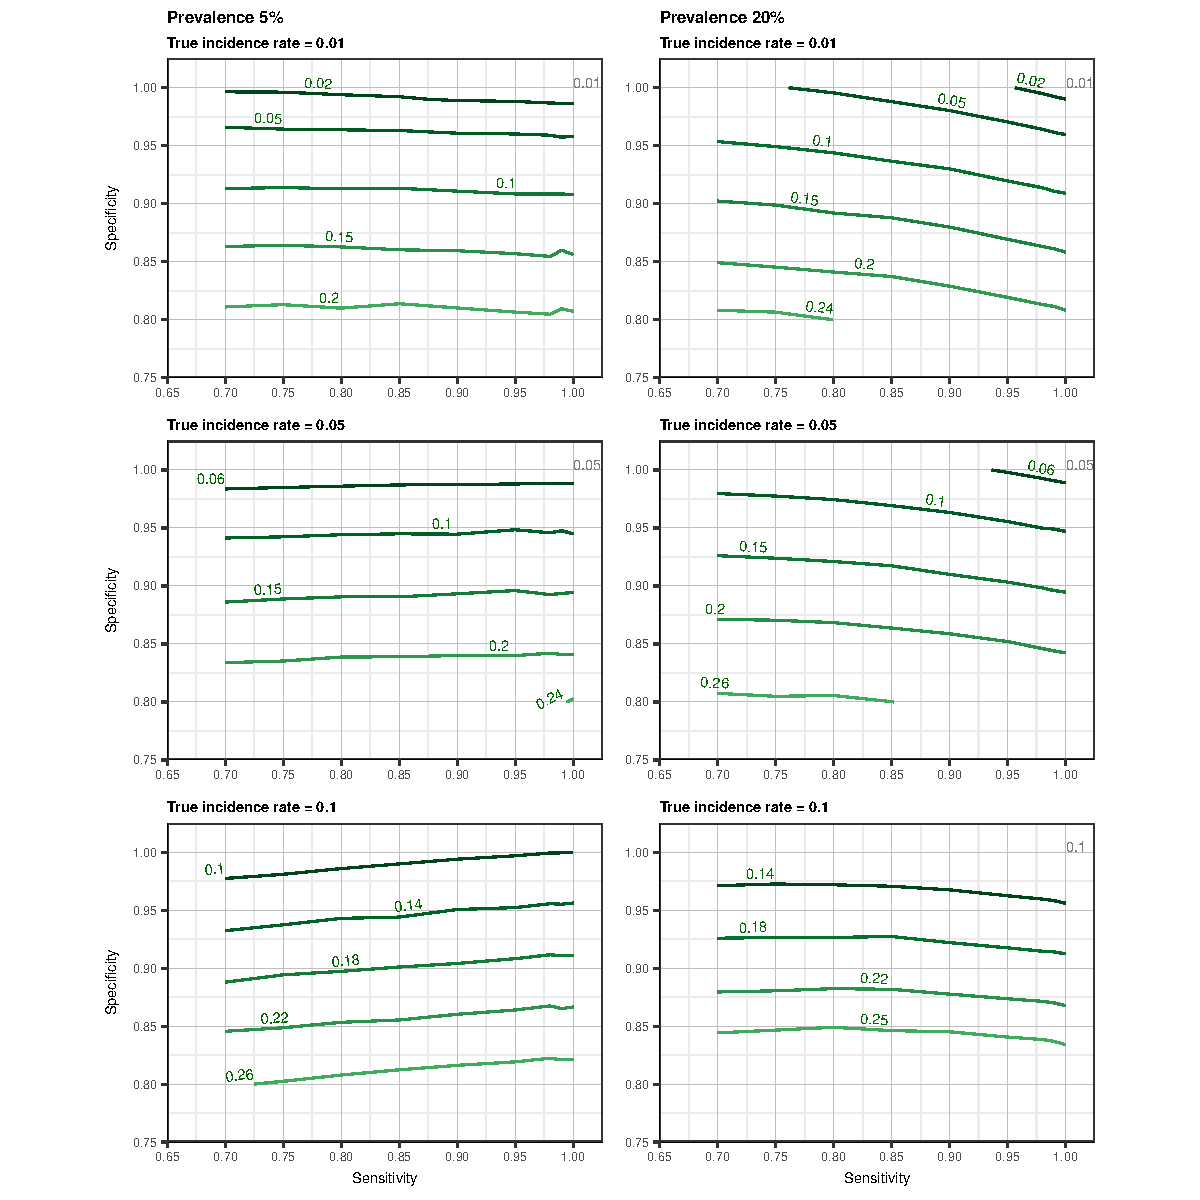
\includegraphics[scale=.95]{master-incidence_contour-1}
    \end{center}
  \caption{Estimated incidence rate (in cases/animal-time unit) as a
function of test sensitivity and specificity, disease prevalence (5 or 20\%),
and true disease incidence (0.01, 0.05, 0.1 case/animal-time unit) when using an
imperfect test both at baseline and follow-up (i.e.\ total bias). True incidence
rate is found at the upper right corner (i.e.\ perfect sensitivity and
specificity).}
  \label{fig:incidence_contour}
\end{figure}

\begin{figure}[htbp]
  \begin{center}
    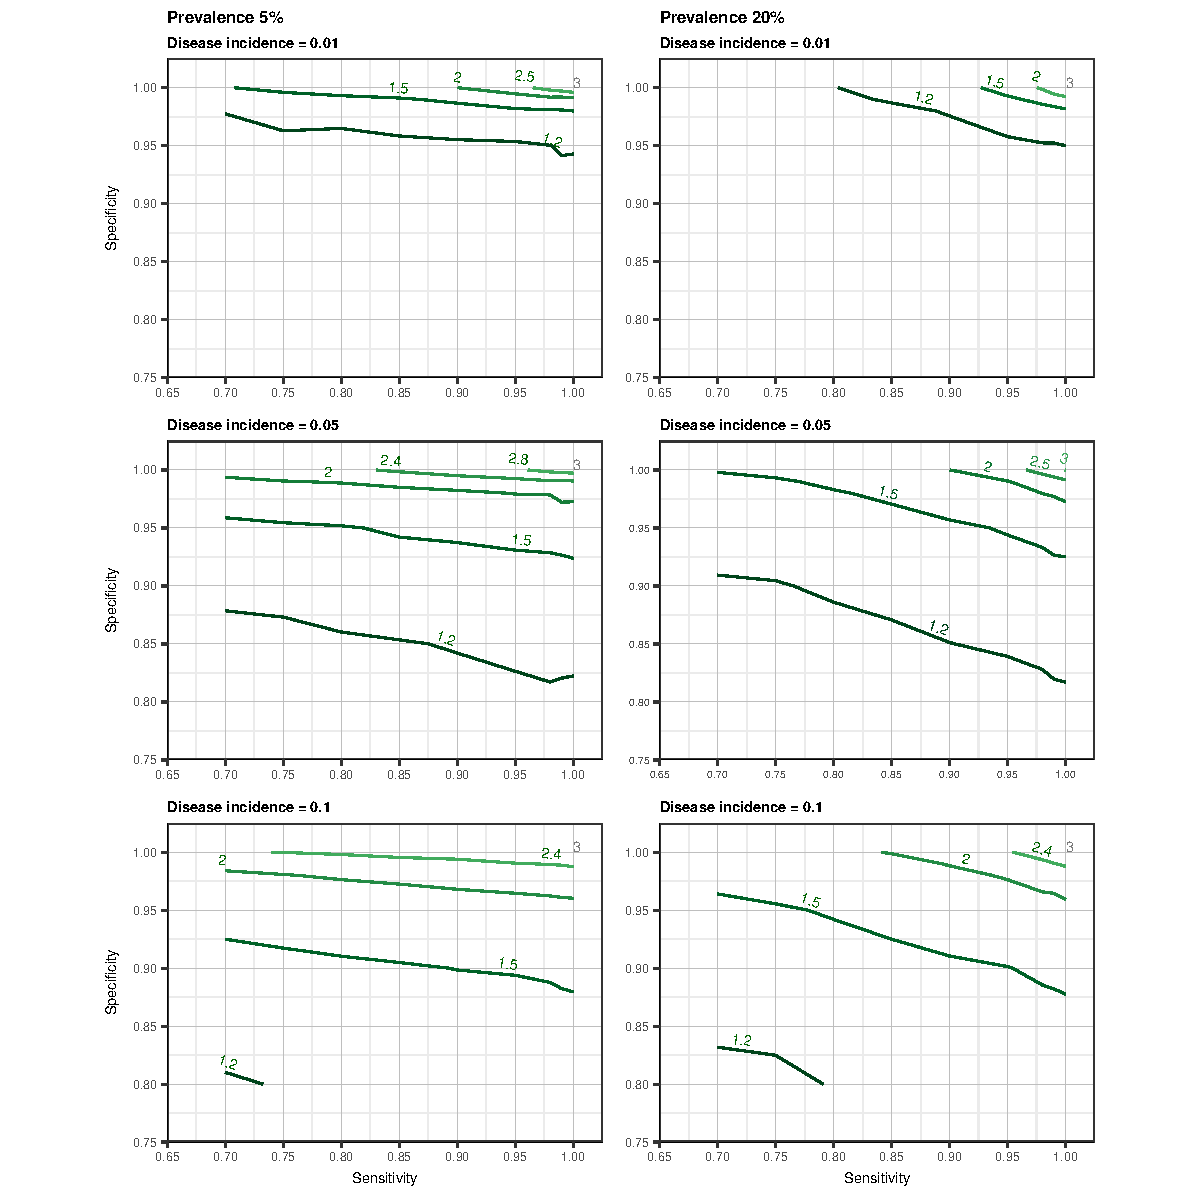
\includegraphics[scale=.95]{master-risk_contour-1}
    \end{center}
  \caption{Estimated risk ratio as a function of test sensitivity and
    specificity, disease prevalence (5 or 20\%), and true disease incidence
    (0.01, 0.05, 0.1 case/animal-time unit) for an exposure with a true measure
    of association corresponding to a risk ratio of \(3.0\) when using an
    imperfect test both at baseline and follow-up (i.e.\ total bias). True risk
    ratio is found at the upper right corner (i.e.\ perfect sensitivity and
    specificity).}
  \label{fig:incidence_risk}
\end{figure}

\begin{figure}[htbp]
  \begin{center}
    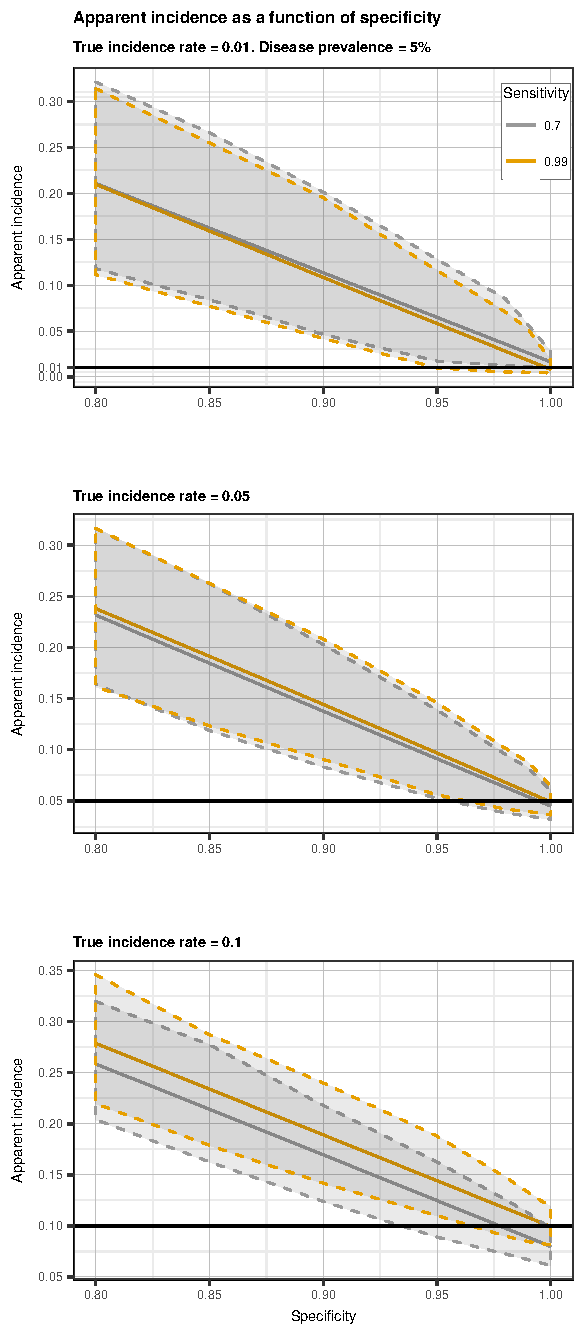
\includegraphics[scale=.95]{master-dohoo5_incidence-1}
    \end{center}
  \caption{Apparent incidence resulting from total bias, as a function of
    specificity. Disease prevalence = 5\%. Solid line: median value; dotted
    lines: first and third quartiles.}
  \label{fig:apparent_incidence_5}
\end{figure}

\begin{figure}[htbp]
  \begin{center}
    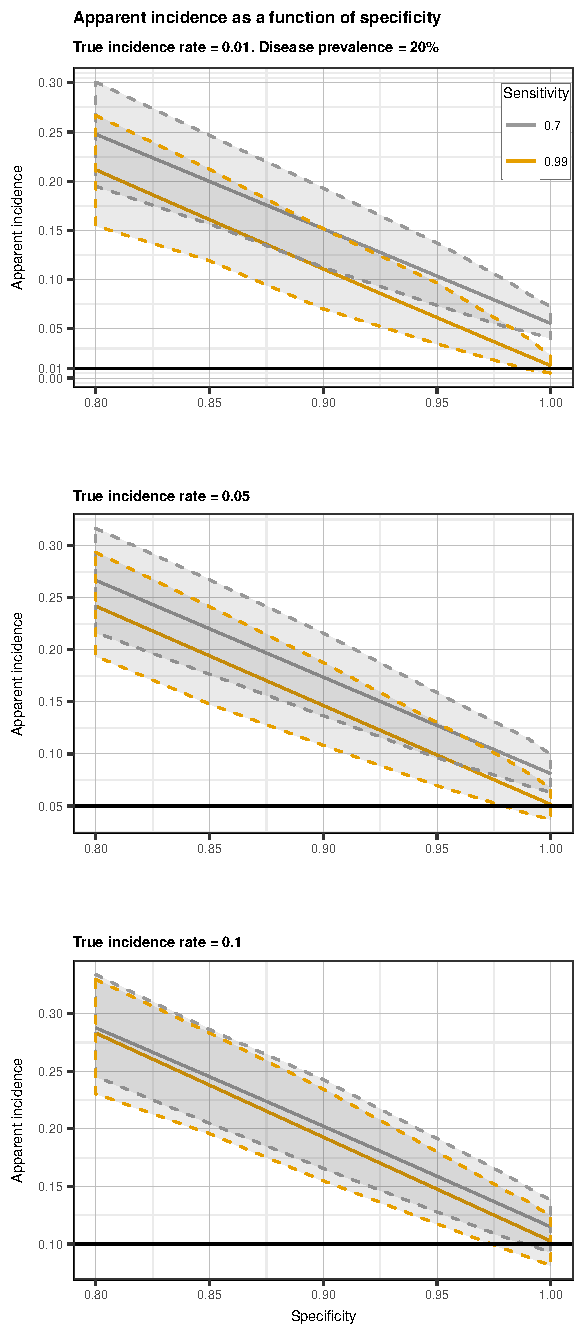
\includegraphics[scale=.95]{master-dohoo20_incidence-1}
    \end{center}
  \caption{Apparent incidence resulting from total bias, as a function of
    specificity. Disease prevalence = 20\%. Solid line: median value; dotted
    lines: first and third quartiles.}
  \label{fig:apparent_incidence_20}
\end{figure}

\begin{figure}[htbp]
  \begin{center}
    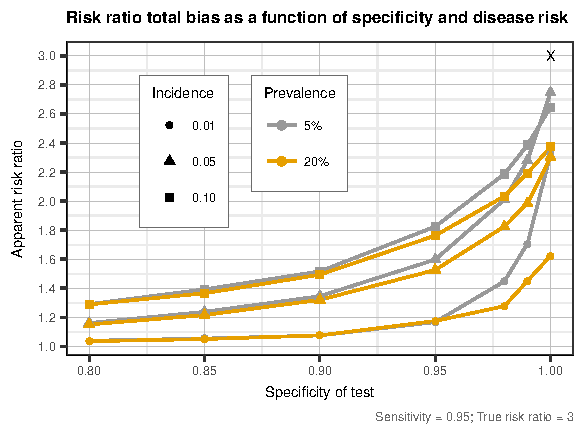
\includegraphics[scale=.95]{master-RR_Se_PrInc-1}
    \end{center}
  \caption{Estimated risk ratio as a function of test specificity and disease
    risk, and for a sensitivity of 95\%, when using an imperfect test both at
    baseline and follow-up. True risk ratio = \(3.0\).}
  \label{fig:apparent_RR}
\end{figure}

%%% If you are submitting a figure with subfigures please combine these into one image file with part labels integrated.
%%% If you don't add the figures in the LaTeX files, please upload them when submitting the article.
%%% Frontiers will add the figures at the end of the provisional pdf automatically
%%% The use of LaTeX coding to draw Diagrams/Figures/Structures should be avoided. They should be external callouts including graphics.

\end{document}

%%% Local Variables:
%%% ispell-local-dictionary: "canadian"
%%% eval: (flyspell-mode 1)
%%% reftex-default-bibliography: ("./bias.bib")
%%% End:
